\chapter{無線センサネットワークにおけるオペレーティングシステム}
\begin{large}
\begin{quote}
本章では,最初にセンサネットワークの一般公衆化を説明し,公衆センサデータ管理における必須な機能要件である地理的探索について述べる.次に,公衆センサデータ管理のシステム設計の際の重要な概念であるデータ管理の時間的密度を解説し,最後にセンサデータの時間的特殊性とそれに起因する公衆センサデータ管理の問題点を述べる.
%本章では、
\end{quote}
\end{large}
\clearpage


%\section{無線センサネットワークにおけるオペレーティングシステム}
%無線センサネットワークのオペレーティングシステムには主に2種類あり、
%イベントモデルとスレッドモデルが存在している。
%無線センサネットワーク用のオペレーティングシステムではイベントモデルが主流となっている。

\section{イベントモデル}
イベントモデルで構築されたオペレーティングシステムは全てのタスクをイベントによって起動し,
run-to-completion で実行する形態のオペレーティングシステムである.
%イベントモデルの動作を図 4 に示す.
イベントモデルはひとつのイベントループと多数のイベントハンドラから構成される.
イベントループはイベントの到着を待ち,
イベントが届くとイベントに関連付けられているイベントハンドラを実行する.
イベントモデルではイベント駆動型プログラミングによってアプリケーションが記述される.
イベントハンドラは寿命の短いrun-to-completionで記述され,
プリエンプションされることがない.
つまり,イベントモデルはタスクは関数呼び出しと等価であり,
実行ストリームがひとつで実現されるため各タスクでローカル変数の領域を共有可能なので
省資源かつ低オーバヘッドで並列性を実現できる.
また,各タスクが不可分に実行されるので共有資源に対する排他制御が不要となり,
安全性が高い.
さらに,CPU の特殊な機能を用いなくても実装できるので移植性も高い.
\begin{figure}[htbp]
 \begin{center}
  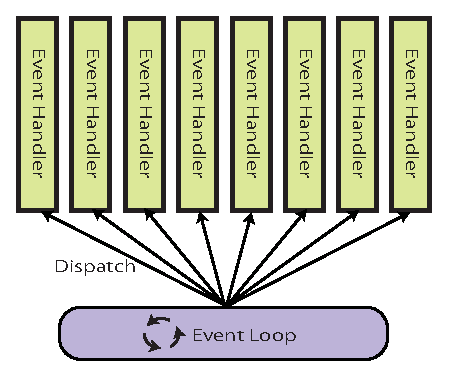
\includegraphics[width=60mm]{./images/event_model.eps}
 \end{center}
 \caption{イベントモデル}
 \label{fig:event_model}
\end{figure}


%\subsection{TinyOS: An Operating System for Sensor Networks}
\subsection{TinyOS}
この中で代表的なものがTinyOS\cite{Hill:2000:SAD:356989.356998}\cite{Levis04tinyos:an}である.
TinyOSはカリフォルニア大学バークレー校のSmartDust Projectで開発されたオペレーティングシステムである.
現在無線センサネットワークの標準的なオペレーティングシステムとして扱われており,
Crossbow社から発売されているMICA2やMICAz\cite{Hill:2002:MWP:623308.624560},
Telos\cite{Polastre:2005:TEU:1147685.1147744},iMote\cite{Nachman:2005:IMP:1147685.1147760}上で動作する.
TinyOSはCPUの特別な機能を使用せずに実装可能であるため,移植性が高く,
ATMELのAVR128LやTexsusのMSP430,ARM7などさまざまなCPUに移植されている.

TinyOSではnesC\cite{Gay:2003:NLH:781131.781133}と呼ばれるイベント駆動型の新しい言語で
複数のイベントハンドラを 1 つのモジュールとして設計可能な機能を提供することで
イベントモデルの持つプログラムの開発のし辛さを提供している.
さらに,nesCはイベント駆動型に特化した最適化を行っているので省資源性も実現される.


%\subsection{A Dynamic Operating System for Sensor Nodes}
\subsection{SOS}
TinyOSがモノリシックなシステムイメージを持っていたのに対し,
SOS\cite{Han:2005:DOS:1067170.1067188}は
イベント駆動型オペレーティングシステムに動的モジュールの機能を実現したものである.
SOSではカーネルから動的モジュールをロードする時に関数の型チェックを行うことで
関数の型違反に伴うバグを防ぐ仕組みを取り入れている.




\section{スレッドモデル}
%スレッドモデルを図 5 に示す.
スレッドモデルは複数のスレッドから構成される.
各スレッドはそれぞれ独立に実行ストリームを持っており,
低い優先度のスレッドは高い優先度のスレッドにプリエンプションされるという特徴を持つ.
スレッドモデルではユーザはあたかもCPUを占有しているかのように
一連の処理をひとつのスレッドとして記述することができるので
プログラムが書きやすい.
また,プリエンプションを行うことも想定しているので
ハードリアルタイム処理をサポートすることができる.
\begin{figure}[htbp]
 \begin{center}
  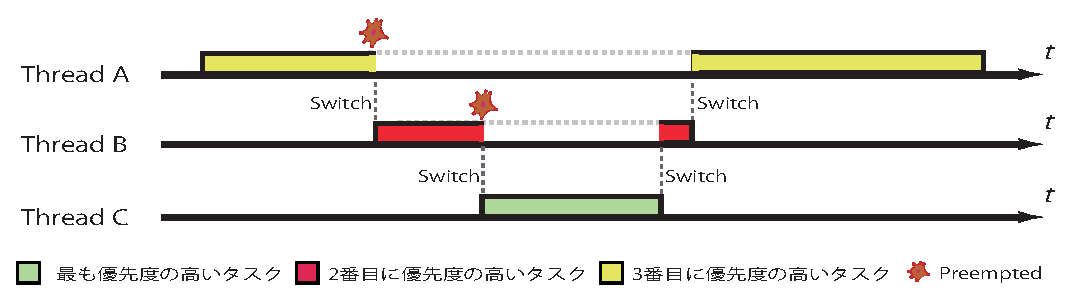
\includegraphics[width=140mm]{./images/threads_model.eps}
 \end{center}
 \caption{スレッドモデル}
 \label{fig:threads_model}
\end{figure}


%\subsection{Nano-RK: an Energy-aware Resource-centric RTOS for Sensor Networks}
\subsection{Nano-RK}



%\subsection{MANTIS OS: An Embedded Multithreaded Operating System for Wireless Micro Sensor Platforms}
\subsection{MANTIS OS}
MANTIS OS\cite{Bhatti:2005:MOE:1160162.1160178}はLinuxやFreeBSDなどで
用いられているスレッドと同様の機能をセンサノード上で
実現したスレッドモデルのオペレーティングシステムである.
開発者はLinuxやFreeBSDなどで用いられているソフトウェアを
大きな変更無しにMANTIS OS上に移植することができる.
また,MANTIS OS上の1つのスレッドとして
TinyOS\cite{Hill:2000:SAD:356989.356998}\cite{Levis04tinyos:an}を
実装することも可能であり\cite{Trumpler06asystematic},
さまざまなソフトウェアリソースをMANTIS OS上で動作可能であることも特徴的である.



%ジョブの実行を設定された時間通りに作動させることをリアルタイム処理という.
%リアルタイム処理には主に
%ハードリアルタイム処理と
%ソフトリアルタイム処理,の2種類がある.
%
%
%\subsection{ハードリアルタイム処理}
%課せられた処理が期限内に終了しなかったとき,
%システム全体に致命的なダメージが生じてしまうリアルタイム処理のことを
%ハードリアルタイム処理という.
%したがって,期限内での終了が保証されなければならないシステムに用いられる.
%
%\subsection{ソフトリアルタイム処理}
%ソフトリアルタイム処理を行うシステムでは,
%期限内に処理が終了しなくてもシステム全体に致命的なダメージを与えることはない.
%ただし,処理自体の価値は終了期限とともに減少していく.


\section{イベントモデルとスレッドモデルの比較}
しかしながら,
ユーザが一連の処理を細かい処理に分割しなければならないのでプログラムが書き辛いという問題が発生する.

さらに,イベントモデルではタスクのプリエンプションをしないことを前提に設計されているので
ハードリアルタイム処理のサポートができない.
しかしながら,プリエンプション時のオーバヘッドの大きいことや必要とされる資源が多いこと,
スレッド間の共有資源へのアクセス制御が必要となるために安全性が損なわれるなどの問題を持っている.

%\begin{table}[htb]
%  \centering
%  \caption{オペレーティングシステムの比較}
%  \begin{tabular}{|c||c|c|c|c|} \hline
%    \backslashbox{}{} & \multicolumn{2}{|c|}{メリット} & \multicolumn{2}{|c|}{デメリット} \\ \hline \hline
%    イベントモデル & 省資源 & 低オーバヘッド & リアルタイム性の非サポート & プログラムが記述しにくい \\ \hline
%    スレッドモデル & \multicolumn{2}{|c|}{リアルタイム性のサポート} & 資源の消費が大きい & 高オーバヘッド \\ \hline
%  \end{tabular}
%  \label{tab:merit_and_demerit}
%\end{table}

\section{まとめ}
本章では,まず,センサネットワークの一般公衆化について述べた.次いで,公衆センサデータがを扱ったシステム設計をする際に,データ管理の時間的密度という要素を考慮すべきであることを示した.そして,センサデータが時間的特殊性を持った多次元データであることを述べ,また,それに起因するセンサデータ管理における問題を提起した.
%システムにおける地理的探索の必要性について記した.さらに,センサデータ以外のコンテンツを扱うシステムとセンサデータを扱うシステムの対比を行い,広域センサデータ管理システムにおけるデータ管理の時間的密度という概念を説明し,最後に,センサデータの時間的特殊性を取り上げた後,それに起因するセンサデータ管理におけるデータ管理の時間的密度の高さという問題を提起した.
